\documentclass[sigconf,screen,natbib=true]{acmart}
%DIF LATEXDIFF DIFFERENCE FILE
%DIF DEL _original/old.tex   Tue Jun  3 04:44:54 2025
%DIF ADD new.tex             Tue Jun  3 04:44:56 2025
\AtBeginDocument{\providecommand\BibTeX{{Bib\TeX}}}

\setcopyright{acmlicensed}
\copyrightyear{2025}
\acmYear{2025}
\acmDOI{XXXXXXX.XXXXXXX}
\acmConference[Conference acronym 'XX]{Make sure to enter the correct
  conference title from your rights confirmation email}{June 03--05,
  2018}{Woodstock, NY}
\acmISBN{978-1-4503-XXXX-X/2018/06}






%
 
\usepackage{subcaption}
\usepackage{enumitem}
\usepackage[most]{tcolorbox}
 %DIF > 
 %DIF > 
 %DIF > 
 %DIF > 
 %DIF > 
\copyrightyear{2025} %DIF > 
\acmYear{2025} %DIF > 
\setcopyright{cc} %DIF > 
\setcctype{by} %DIF > 
\acmConference[COMPASS '25]{ACM SIGCAS/SIGCHI Conference on Computing and Sustainable Societies}{July 22--25, 2025}{Toronto, ON, Canada} %DIF > 
\acmBooktitle{ACM SIGCAS/SIGCHI Conference on Computing and Sustainable Societies (COMPASS '25), July 22--25, 2025, Toronto, ON, Canada} %DIF > 
\acmDOI{10.1145/3715335.3736327} %DIF > 
\acmISBN{979-8-4007-1484-9/2025/07} %DIF > 
%DIF PREAMBLE EXTENSION ADDED BY LATEXDIFF
%DIF UNDERLINE PREAMBLE %DIF PREAMBLE
\RequirePackage[normalem]{ulem} %DIF PREAMBLE
\RequirePackage{color}\definecolor{RED}{rgb}{1,0,0}\definecolor{BLUE}{rgb}{0,0,1} %DIF PREAMBLE
\providecommand{\DIFadd}[1]{{\protect\color{blue}\uwave{#1}}} %DIF PREAMBLE
\providecommand{\DIFdel}[1]{{\protect\color{red}\sout{#1}}} %DIF PREAMBLE
%DIF SAFE PREAMBLE %DIF PREAMBLE
\providecommand{\DIFaddbegin}{} %DIF PREAMBLE
\providecommand{\DIFaddend}{} %DIF PREAMBLE
\providecommand{\DIFdelbegin}{} %DIF PREAMBLE
\providecommand{\DIFdelend}{} %DIF PREAMBLE
\providecommand{\DIFmodbegin}{} %DIF PREAMBLE
\providecommand{\DIFmodend}{} %DIF PREAMBLE
%DIF FLOATSAFE PREAMBLE %DIF PREAMBLE
\providecommand{\DIFaddFL}[1]{\DIFadd{#1}} %DIF PREAMBLE
\providecommand{\DIFdelFL}[1]{\DIFdel{#1}} %DIF PREAMBLE
\providecommand{\DIFaddbeginFL}{} %DIF PREAMBLE
\providecommand{\DIFaddendFL}{} %DIF PREAMBLE
\providecommand{\DIFdelbeginFL}{} %DIF PREAMBLE
\providecommand{\DIFdelendFL}{} %DIF PREAMBLE
%DIF COLORLISTINGS PREAMBLE %DIF PREAMBLE
\RequirePackage{listings} %DIF PREAMBLE
\RequirePackage{color} %DIF PREAMBLE
\lstdefinelanguage{DIFcode}{ %DIF PREAMBLE
%DIF DIFCODE_UNDERLINE %DIF PREAMBLE
  moredelim=[il][\color{red}\sout]{\%DIF\ <\ }, %DIF PREAMBLE
  moredelim=[il][\color{blue}\uwave]{\%DIF\ >\ } %DIF PREAMBLE
} %DIF PREAMBLE
\lstdefinestyle{DIFverbatimstyle}{ %DIF PREAMBLE
	language=DIFcode, %DIF PREAMBLE
	basicstyle=\ttfamily, %DIF PREAMBLE
	columns=fullflexible, %DIF PREAMBLE
	keepspaces=true %DIF PREAMBLE
} %DIF PREAMBLE
\lstnewenvironment{DIFverbatim}{\lstset{style=DIFverbatimstyle}}{} %DIF PREAMBLE
\lstnewenvironment{DIFverbatim*}{\lstset{style=DIFverbatimstyle,showspaces=true}}{} %DIF PREAMBLE
\lstset{extendedchars=\true,inputencoding=utf8}

%DIF END PREAMBLE EXTENSION ADDED BY LATEXDIFF

\begin{document}

\title{The~Air~We~Share:~Seven-Month~Mixed~Method~Study~of Thailand's~Motorcycle~Rideshare~Driver~and~Air~Pollution}



\author{Nussara Tieanklin}
\orcid{0000-0002-3074-8699}
\email{nussara@cs.washington.edu}
\affiliation{\institution{University of Washington}
 \city{Seattle}
 \state{Washington}
 \country{USA}
}


\author{Chanwut Kittivorawong}
\orcid{0000-0002-2884-2221}
\DIFdelbegin %DIFDELCMD < \email{chanwutk@berkeley.edu}
%DIFDELCMD < %%%
\DIFdelend \DIFaddbegin \email{chanwutk@cs.berkeley.edu}
\DIFaddend \affiliation{\institution{University of California, Berkeley}
  \city{Berkeley}
  \state{California}
  \country{USA}
}


\author{Joseph Breda}
\orcid{0000-0002-2795-7334}
\email{joebreda@cs.washington.edu}
\affiliation{\institution{University of Washington}
 \city{Seattle}
 \state{Washington}
 \country{USA}
}




\author{Adisorn Lertsinsrubtavee}
\orcid{0000-0002-3814-5913}
\email{adisorn@ait.ac.th}
\affiliation{\institution{Asian Institute of Technology}
 \city{Bangkok}
 \country{Thailand}
}

\author{Preechai Mekbungwan}
\orcid{0000-0002-6444-9857}
\email{preechaim@ait.ac.th}
\affiliation{\institution{Asian Institute of Technology}
 \city{Bangkok}
 \country{Thailand}
}


\author{Raunak Mukhia}
\orcid{0009-0002-6277-8881}
\email{rmukhia@ait.ac.th}
\affiliation{\institution{Asian Institute of Technology}
 \city{Bangkok}
 \country{Thailand}
}


\author{Kalana G.S. Jayarathna}
\orcid{0000-0001-5265-2260}
\email{kalana@ait.ac.th}
\affiliation{\institution{Asian Institute of Technology}
 \city{Bangkok}
 \country{Thailand}
}


\author{Ratchaphon Samphutthanont}
\orcid{0009-0003-7804-5356}
\email{ratchaphon_sam@cmru.ac.th}
\affiliation{\institution{Chiang Mai Rajabhat University}
 \city{Chiang Mai}
 \country{Thailand}
}


\author{Chayanon Sawatdeenarunat}
\orcid{0000-0001-9266-7176}
\email{chayanon@cmru.ac.th}
\affiliation{\institution{Chiang Mai Rajabhat University}
 \city{Chiang Mai}
 \country{Thailand}
}

\author{Kurtis Heimerl}
\orcid{0000-0002-0989-5440}
\email{kheimerl@cs.washington.edu}
\affiliation{\institution{University of Washington}
 \city{Seattle}
 \state{Washington}
 \country{USA}
}
 \newtcolorbox{quack}{
  breakable,
  enhanced,
  frame hidden,
  interior hidden,
  size=minimal,
  left skip=-3pt,
  borderline west={1.5pt}{-8pt}{lightgray}
}

\newenvironment{quoteb}{\begin{quote}\begin{quack}}{\end{quack}\end{quote}}

\newcommand{\joe}[1]{\textcolor{cyan}{[Joe: #1]}}
\newcommand{\mick}[1]{\textcolor{olive}{[mick: #1]}}
\newcommand{\kurtis}[1]{\textcolor{purple}{[#1 -k]}}
\newcommand{\firn}[1]{\textcolor{orange}{[firn: #1]}}
\newcommand{\todo}[1]{\textcolor{red}{[TODOs: #1]}}
\newcommand{\reread}[1]{\textcolor{blue}{[reread: #1]}}


\DIFdelbegin %DIFDELCMD < \newcommand{\grab}[1]{\textsc{RideshareCompanyA}}
%DIFDELCMD < %%%
\DIFdelend \DIFaddbegin \newcommand{\grab}[1]{\textcolor{red}{\textsc{RideshareCompanyA}}}
\DIFaddend 

\renewcommand{\shortauthors}{Tieanklin et al.}


\newcommand{\para}[1]{\paragraph{\bf\em #1}} \begin{abstract}



Addressing the gap between gig work autonomy and environmental health agencies, this study investigates extreme PM2.5 exposure among motorcycle rideshare drivers in urban Thailand.
These workers face high risks due to prolonged open-air work with extensive working hours, often rendering standard health advice impractical.
Using a mixed-methods approach combining seven months of longitudinal personal PM2.5 data and qualitative interviews,
we captured detailed exposure patterns and explored lived experiences, health perceptions, coping strategies, and systemic barriers.
We find drivers are consistently exposed to PM2.5 exceeding guidelines,
with limited agency to mitigate these risks due to economic necessity and structural constraints.
Our research underscores the critical need for interventions targeting exposure reduction and worker empowerment,
balancing health protection with income stability for this vulnerable population.


\end{abstract} 









%

\maketitle

\section{Introduction}

\DIFaddbegin \todo{The research questions this study is trying to answer is not clearly stipulated.}





\DIFaddend Motorcycle rideshare drivers in Thailand, often low-income, face prolonged outdoor work in dense, polluted urban areas \cite{tieanklin2024rideshare}.
This vulnerability is amplified by high motorcycle usage (87\% of households in 2014 \cite{Poushter2015motorcyclestat}) and poor air quality \cite{iqr_rank}.
A key hazard is PM2.5, fine particulate matter linked to severe health risks, including respiratory and cardiovascular diseases and millions of premature deaths globally \cite{who_ambient_air_pollution}.
Prolonged exposure is associated with a 6-13\% increase in heart disease mortality per 10 $\mu g/m^3$ of PM2.5.

Standard public health advice for high PM2.5 (e.g., stay indoors and avoid busy roads) \cite{cdc_pm25} is often impractical for these workers.
Financial pressures and platform dynamics limit their agency to prioritize health over income, creating a gap between known risks and self-protection capabilities \cite{tieanklin2024rideshare}.







Understanding the specific, individual experiences of PM2.5 exposure and the barriers preventing workers from prioritizing their health is crucial.
This study aims to bridge this gap by focusing on the lived experiences of at-risk workers (including but not limited to rideshare drivers) in urban Thailand.
We employ a methodology combining longitudinal personal sensing with qualitative interviews to capture both the quantitative patterns and the qualitative nuances of exposure and agency over seven months.
By deploying personal sensors, we gather detailed, real-time data on individual PM2.5 exposure across varying conditions.
This quantitative data is complemented by in-depth qualitative interviews exploring personal narratives, health perceptions, and coping strategies.
We will present data illustrating that workers frequently experience exposure exceeding WHO guidelines \cite{who_aqg_2021}, highlighting the urgency of this issue.








Key contributions include:
\begin{enumerate}
    \item 
Fine-grained, longitudinal individual PM2.5 exposure monitoring.
    \item 
Integration of sensor data with qualitative insights into lived experiences and perceptions relative to health guidelines.
    \item 
Identifying challenges, coping strategies, and agency constraints through worker narratives.
    \item 
Exploring potential solutions considering health-income trade-offs. This research aims to inform interventions enhancing worker agency and well-being.
\end{enumerate}




























%
 \section{Related Work}
We review prior work on air pollution exposure, socio-economic disparities, and impacts on motorcycle rideshare workers.
\DIFaddbegin \todo{The related work section lacks depth; only four studies have been included in this section. It would be good if it included more studies that have studied a related phenomenon and synthesised how these studies inform the current study}
\mick{probably don't have time to find+add more related work}
\DIFaddend 

\subsection{Rideshare Workers and Their Agency to Prioritize Health}




Tieanklin et al.~\cite{tieanklin2024rideshare} found that Thai motorcycle rideshare drivers often prioritize income over health despite pollution awareness.
While gig work offers flexibility, financial/social pressures and ride assignment opacity limit their agency to avoid pollution~\cite{machado2021midlife,elfassy2019associations}.
Our longitudinal study provides deeper temporal insights into these dynamics.
By incorporating hyperlocal data with real-time air quality monitoring sensors, we offer a granular understanding of the environmental challenges faced by these gig workers, enhancing public health perspectives.






\subsection{Air pollution in Bangkok, Thailand}
Nguyen et al.~\cite{nguyen2023bangkokpollution} linked socio-economic status (SES) to air pollution exposure and health impacts in Bangkok, finding that informal workers were highly affected and public awareness was low or misaligned with official data.
Building on the findings on socio-economic inequality and public perceptions regarding air pollution, we focus on motorcycle drivers—a highly exposed, low-SES group.
Our study measures their hyperlocal air pollution exposure and uses interviews to explore how their perceptions influence decision-making.

 \section{Methodology}

This study combined real-time sensor deployment for hyperlocal air pollution monitoring with qualitative interviews capturing participant experiences and perceptions.
University of Washington Institutional Review Board (IRB) approval was obtained.

\subsection{Participants Recruitment}

Ten adult motorcycle rideshare drivers (five each from Bangkok/Chiang Mai) were recruited to capture diverse driving behaviors and exposure patterns.
Inclusion criteria were regular passenger transport and driving $\ge$5 hours/day; passengers-dropoff drivers were preferred.
Participant income details are in \autoref{tab:demo}.


\begin{table}[ht]
    \centering
    \caption[Participant Income]{Participant income sources (Rideshare: \DIFdelbeginFL %DIFDELCMD < \grab{}%%%
\DIFdelendFL \DIFaddbeginFL \DIFaddFL{app-based}\DIFaddendFL ; Legacy: station-based) and self-estimated daily average (THB).
    DriverID prefix indicates location (BKK: Bangkok, CMI: Chiang Mai).}
    \begin{tabular}{|c|l|c|}
        \hline
        \textbf{DriverID} & \textbf{Source of Income} & \textbf{Avg. Income/} \\
         &  & \textbf{Day (THB)} \\
        \hline
        BKK1  & Rideshare, Legacy & 2250 \\
        BKK2  & Legacy & 800 \\
        BKK3  & Rideshare, Legacy & 1300 \\
        BKK4  & Rideshare, Legacy & 1350 \\
        BKK5  & Rideshare & 1800 \\
        CMI1  & Rideshare & 700 \\
        CMI2  & Rideshare & 700 \\
        CMI3  & Rideshare & 600 \\
        CMI4  & Small Business Owner, Rideshare & 500 \\
        CMI5  & Rideshare & 900 \\
        \hline
    \end{tabular}
\label{tab:demo}
\end{table}

In Bangkok, participants were initially recruited through a widely used motorcycle ride-hailing application. 
Drivers were approached during rides, with an author (a native Thai speaker) explaining the study objectives and eligibility criteria. 
Due to last-minute participant dropouts, the research team recruited an additional motorcycle rideshare driver from the legacy rideshare system, where drivers wait for passengers at designated stations. 


In Chiang Mai, due to fewer rideshare drivers, recruitment occurred via an \DIFdelbegin \DIFdel{informal }%DIFDELCMD < \grab{} %%%
\DIFdelend \DIFaddbegin \DIFadd{unofficial rideshare }\DIFaddend driver association.


\paragraph{On-boarding Process}


Interested drivers received study details (purpose, procedures, data handling) and provided informed consent.
Participants were required to sign an informed consent form before participating in the study.
Participants were trained on accessing/interpreting their real-time data via a map visualization~\cite{mapvis}.
We clarified non-affiliation with rideshare platforms and informed participants of their right to withdraw or request data deletion anytime without penalty.








\paragraph{Compensation}
Participants were compensated 4,000 Baht per month for their participation, with payments distributed twice monthly during check-ins by transferring into their bank account.

\subsection{Real-Time Sensor Deployment and Calibration}

To collect real-time air pollution data, we deployed 10 portable low-cost air quality sensors developed by our research team.
\DIFaddbegin \mick{cite here?}
\DIFaddend 

\DIFaddbegin \DIFadd{To ensure accuracy, each sensor was field-tested by co-locating it with a reference air quality station operated by Thailand’s Pollution Control Department (PCD) in Bangkok.
Over five days, three low-cost sensors showed strong alignment with hourly PM2.5 readings from the PCD station, with Pearson correlation coefficients consistently above 0.81, indicating high reliability.
}







\DIFaddend \paragraph{Sensor Deployment and Support}
Sensors were mounted on helmets of 10 motorcycle \DIFdelbegin \DIFdel{taxi }\DIFdelend \DIFaddbegin \DIFadd{rideshare }\DIFaddend drivers (5 Chiang Mai, 5 Bangkok) near the breathing zone, powered by 2 portable batteries during their 6-17 hour workdays.
Drivers manually operated sensors and used a LINE group (a popular messaging app in Thailand) for communication and troubleshooting assistance, prompted by automated malfunction notifications.
They could view real-time collective data via a web application featuring a map visualization tool~\cite{mapvis} displaying color-coded pollution levels; training was provided.
Deployment spanned November 2023 to mid-May 2024, covering Thailand's peak pollution season (Jan-Apr) and diverse seasonal conditions to capture varied PM2.5 exposure.

\paragraph{Bi-Weekly Check-Ins}
Biweekly check-ins facilitated participant feedback, shared data summaries (local street-level pollution), equipment checks, and re-calibration.






\subsection{Qualitative Interview}

Qualitative exit interviews with all participants explored their experiences, routines, and perceptions of air pollution (pre/post study).
Conducted by a native Thai author, the 45-60 minute semi-structured interviews used open-ended questions. 


\paragraph{Interview Coding}




We analyzed qualitative data using thematic analysis \cite{braun2006using}, collaboratively developing a codebook via inductive and deductive approaches \cite{saldana2021coding,kathleen2008team}.
Interviews, transcribed in Thai, were iteratively coded for recurring themes.
Two researchers independently coded a subset of transcripts for inter-coder reliability and resolved discrepancies through discussion.
Key themes included changes in driver awareness of air pollution, behavior changes during high PM2.5 periods, and \DIFdelbegin \DIFdel{challenges using the sensor helmet}\DIFdelend \DIFaddbegin \DIFadd{participants' engagement in the project}\DIFaddend .
We then applied axial coding using the codebook to explore theme interrelationships \cite{williams2019art}.


 

\section{Overview of Collected Data}
\label{sec:result-overview-data}

\paragraph{Air Quality Data From Sensors}
Over the seven-month period (November 2023 to mid-May 2024), we collected data from ten motorcycle \DIFdelbegin \DIFdel{taxi }\DIFdelend \DIFaddbegin \DIFadd{rideshare }\DIFaddend drivers in Bangkok and Chiang Mai, covering peak and non-peak pollution seasons.
Each driver wore a helmet-mounted low-cost PM2.5 sensor, calibrated against stationary PCD air quality towers in Chiang Mai and Bangkok.
In total, we captured over 50 million data points on street-level pollution in approximately 163.49 km$^2$ driven in Bangkok and 97.21 km$^2$ in downtown Chiang Mai.
Drivers drive approximately 6-10 hours per day, with consistent sensor functionality powered by portable power banks.
\DIFaddbegin \mick{make sure to link the github repo containing the data}
\DIFaddend 

\DIFaddbegin \todo{The authors could have elaborated on what was contained in the 50 million data points, what data work was conducted to ensure the data was good enough}
\mick{What did we do to clean the data?}





\DIFaddend \paragraph{Exit Interviews}
We conducted qualitative exit interviews with all participants to supplement the sensor data. 
These interviews focused on understanding drivers' experiences with sensor-equipped helmets, their daily driving patterns, and any changes in awareness or behavior regarding air pollution. 
The author, a native Thai speaker, conducted the 60-90 minute interviews, using a semi-structured approach with open-ended questions.  \section{Results}


This section analyzes the collective behaviors of motorcycle taxi drivers using helmet-mounted sensor data (air quality, location, movement) to understand how individual PM2.5 exposure varies across time periods and locations, and how drivers subsequently respond based on these observed exposure patterns.

\begin{figure*}
    \centering
    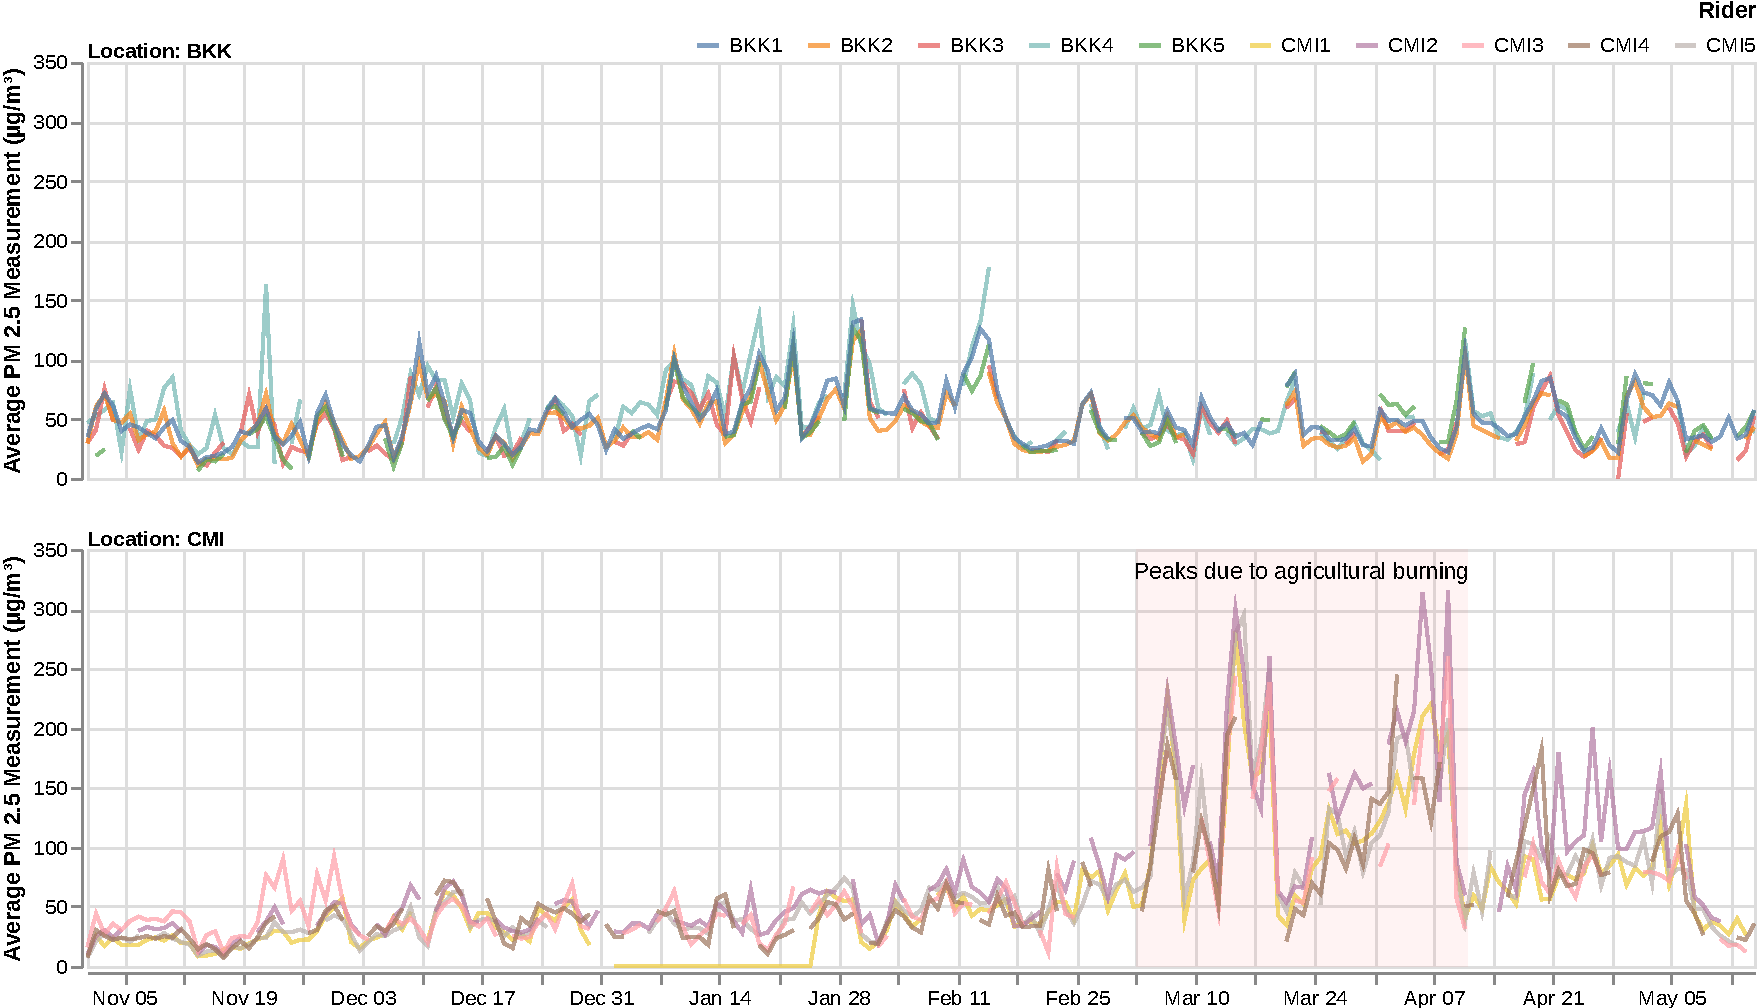
\includegraphics[width=\textwidth]{figures/daily-pollution-per-rider.pdf}
    \caption{
    Daily PM 2.5 exposure measured from the helmet-mounted sensors for Bangkok and Chiang Mai drivers.
    Vertical grid lines represent Sundays.
    }
    \Description{}
    \label{fig:daily-pollution-per-driver}
\end{figure*}

\subsection{PM2.5's Temporal Patterns}
Analyzing daily average PM2.5 exposure (\autoref{fig:daily-pollution-per-driver}) reveals relatively consistent levels in Bangkok (BKK), peaking moderately from December to mid-February,
while Chiang Mai (CMI) shows pronounced seasonality with extreme peaks from March to early April (consistent with agricultural burning periods~\cite{david2025chiangmaiburn, bernsten2024chiangmaiburn, iqair2023chiangmaiburn}).
Within each city, drivers experience similar daily trends.
Hourly averages (\autoref{fig:hourly-work-aqi}) show daily cycles peaking during morning (BKK: 7 AM, CMI: 8 AM) and evening rush hours, with an afternoon dip, although late night/early morning data shows higher variance.
Notably, BKK's PM2.5 measurements show a consistent trend throughout the year, reinforcing traffic as the primary air pollution source.
In contrast, CMI's dominant seasonal variation indicates agricultural burning as the primary driver.
Thus, PM2.5 sources differ substantially between cities (BKK: traffic, CMI: agricultural burning), implying the need for location-specific mitigation strategies.





\begin{figure*}
    \centering
    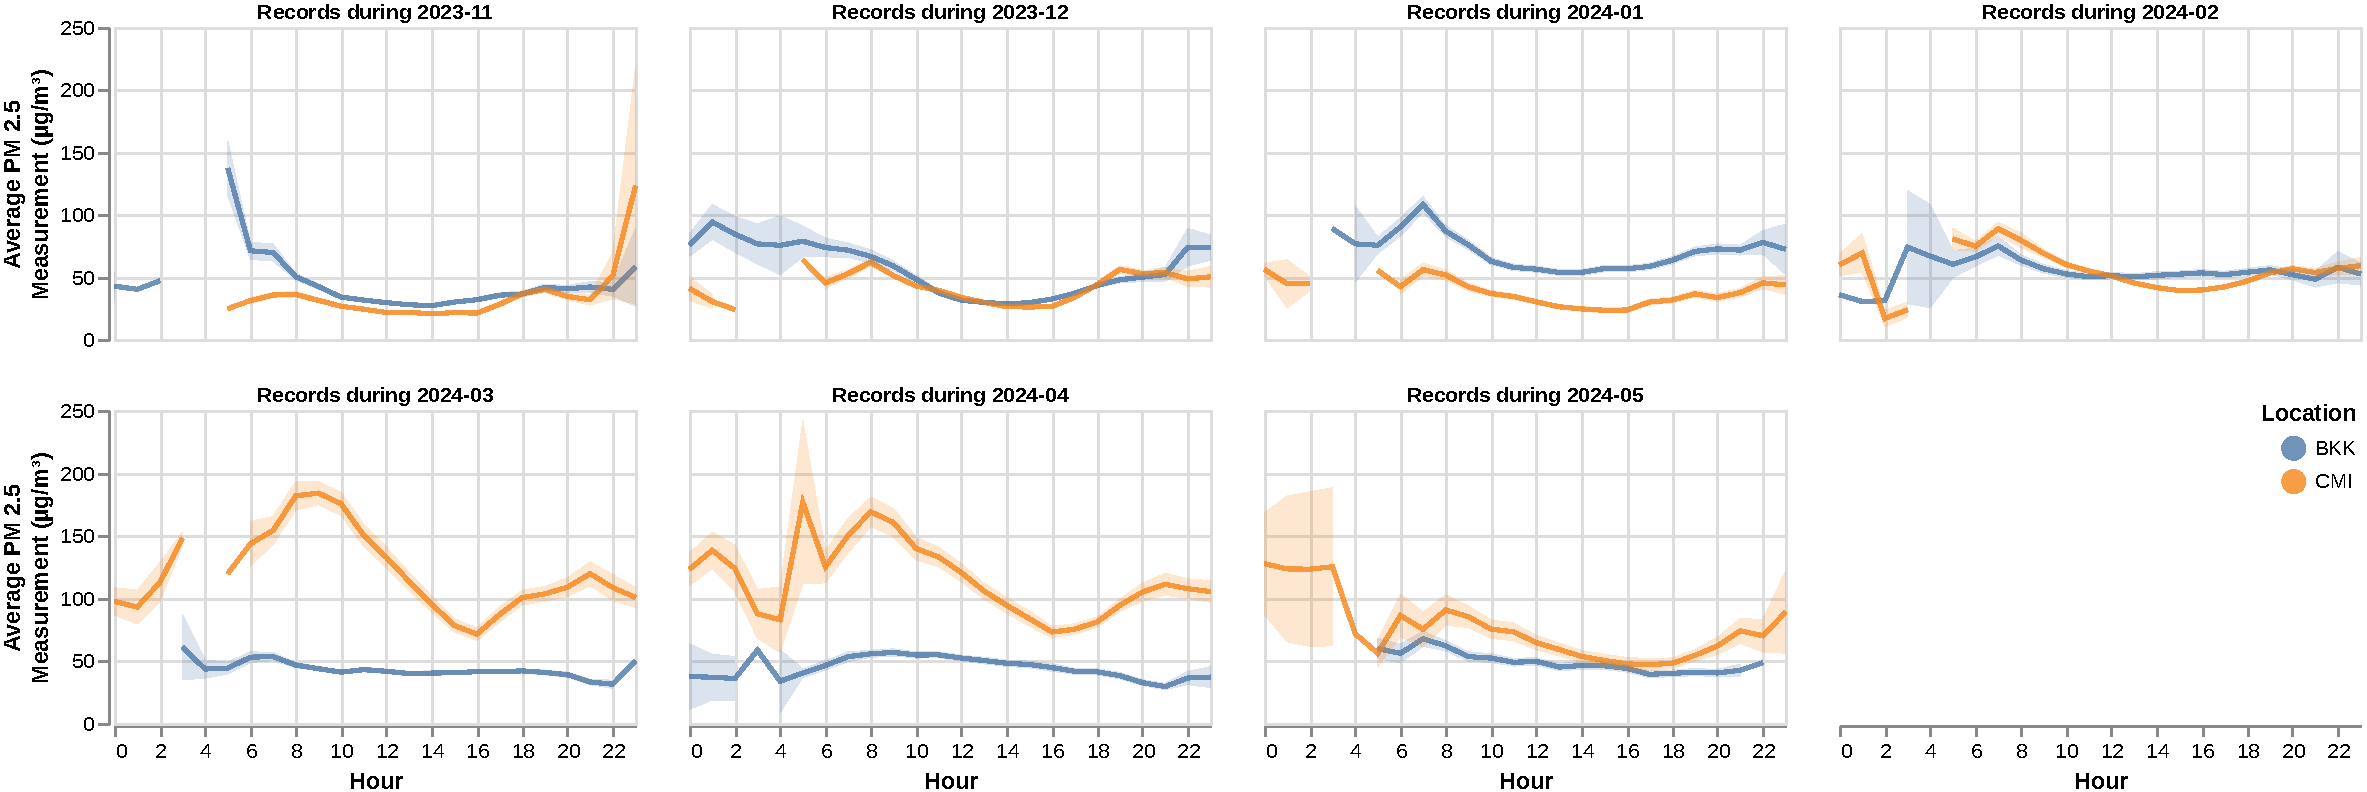
\includegraphics[width=\textwidth]{figures/average-hourly-pollution.pdf}\caption{Mean and standard deviations of air pollution measurement in each hour of the day throughout the study period.
Each subplot represents each month in the study. }\Description{}
    \label{fig:hourly-work-aqi}\end{figure*}





\subsection{PM2.5's Spatial Patterns}


Spatial analysis (\autoref{fig:subdistrict-aqi}) reveals that PM2.5 distribution is uneven across subdistricts and individual drivers, with drivers experiencing different exposure levels even in similar areas.
Furthermore, each driver tends to operate primarily within specific locations.
Consequently, effective PM2.5 exposure mitigation strategies must consider these individual spatial work patterns.


\begin{figure*}
    \centering
    \begin{subfigure}[t]{0.49\textwidth}
        \centering
        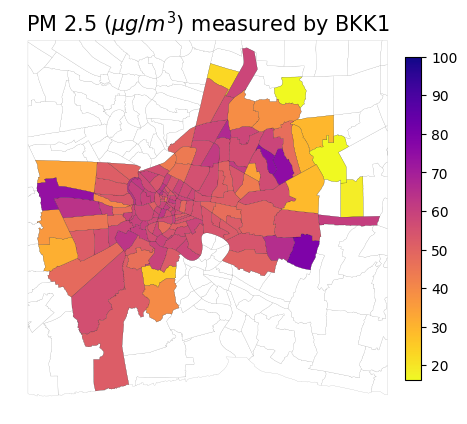
\includegraphics[width=.5\linewidth]{figures/map/BKK1_PM25.png}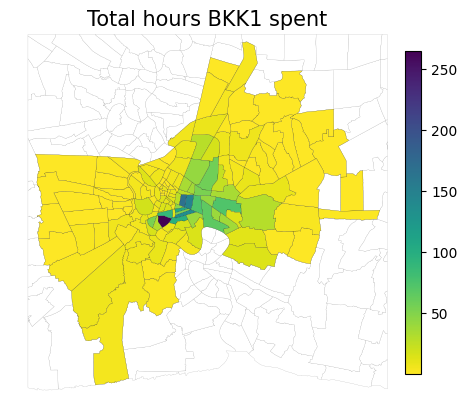
\includegraphics[width=.5\linewidth]{figures/map/BKK1_time.png}
        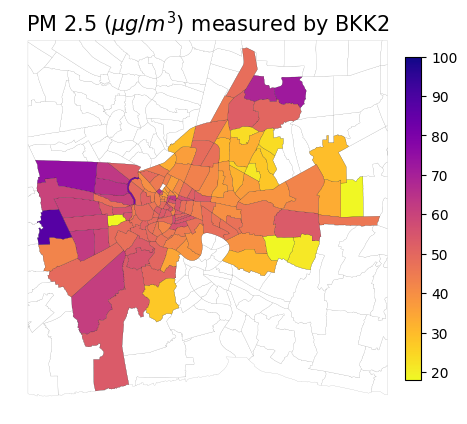
\includegraphics[width=.5\linewidth]{figures/map/BKK2_PM25.png}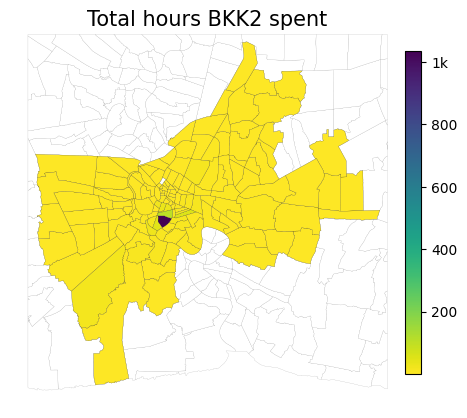
\includegraphics[width=.5\linewidth]{figures/map/BKK2_time.png}
        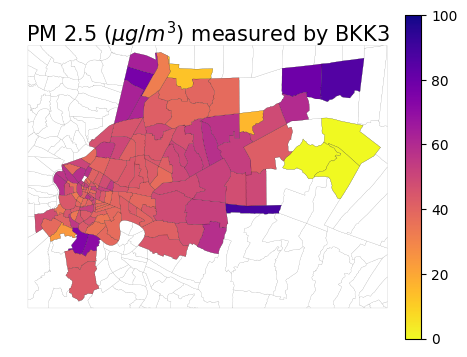
\includegraphics[width=.5\linewidth]{figures/map/BKK3_PM25.png}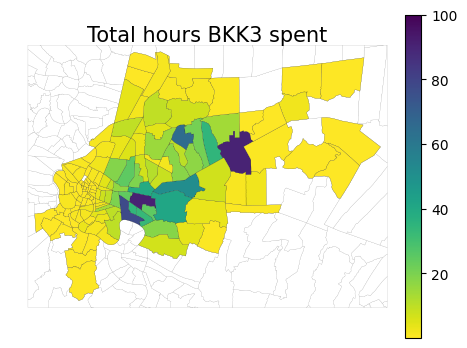
\includegraphics[width=.5\linewidth]{figures/map/BKK3_time.png}
        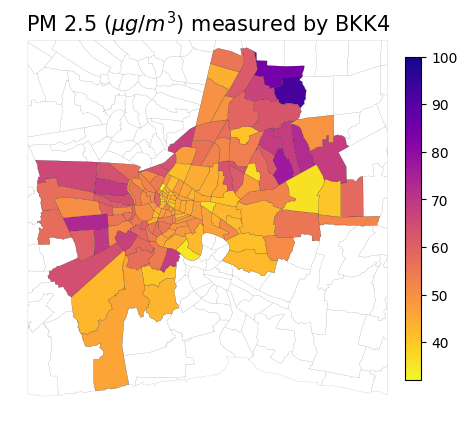
\includegraphics[width=.5\linewidth]{figures/map/BKK4_PM25.png}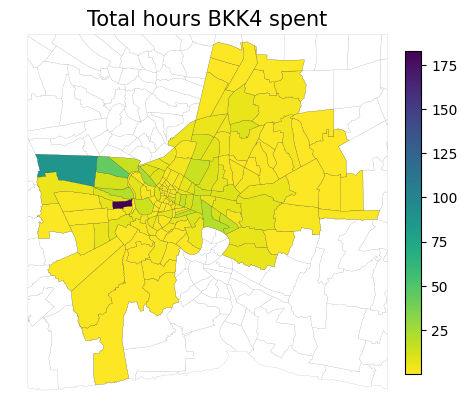
\includegraphics[width=.5\linewidth]{figures/map/BKK4_time.png}
        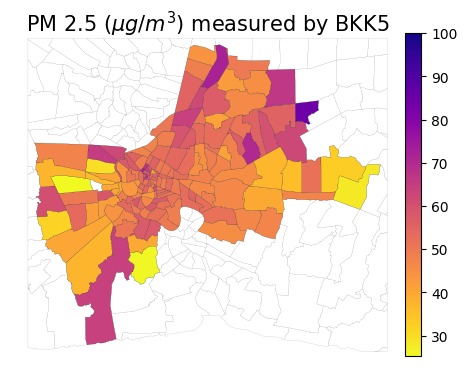
\includegraphics[width=.5\linewidth]{figures/map/BKK5_PM25.png}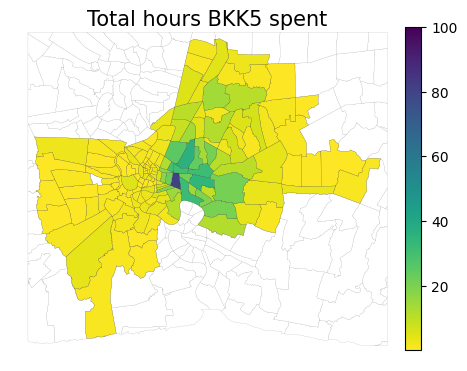
\includegraphics[width=.5\linewidth]{figures/map/BKK5_time.png}
        \caption{Measurement collected in Bangkok.}
\end{subfigure}\hfill \begin{subfigure}[t]{0.49\textwidth}
        \centering
        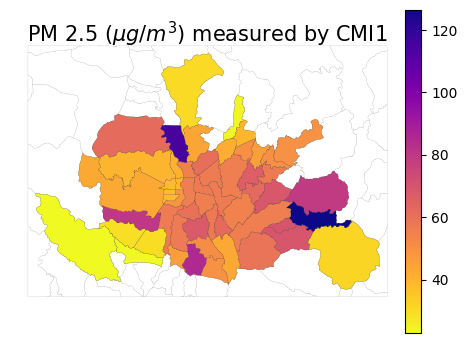
\includegraphics[width=.5\linewidth]{figures/map/CMI1_PM25.png}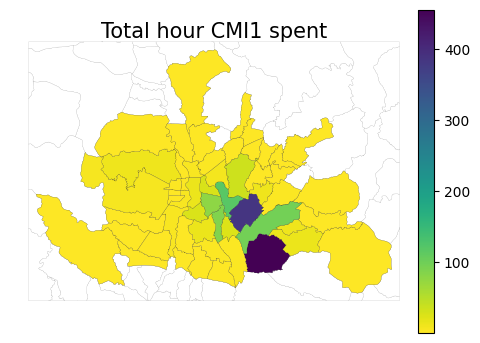
\includegraphics[width=.5\linewidth]{figures/map/CMI1_time.png}
        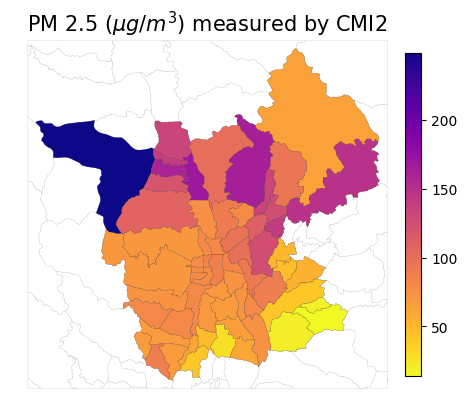
\includegraphics[width=.5\linewidth]{figures/map/CMI2_PM25.png}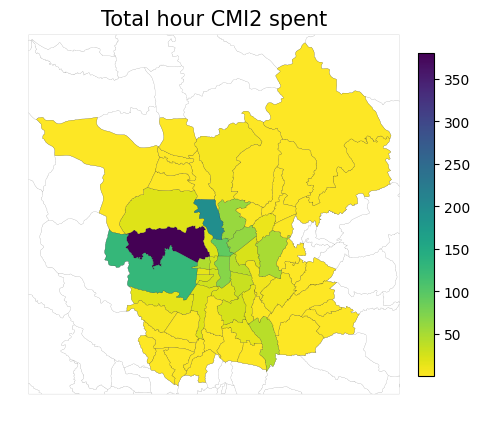
\includegraphics[width=.5\linewidth]{figures/map/CMI2_time.png}
        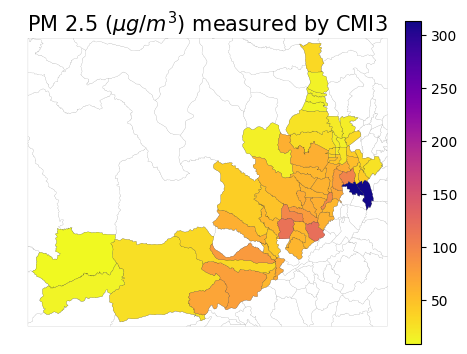
\includegraphics[width=.5\linewidth]{figures/map/CMI3_PM25.png}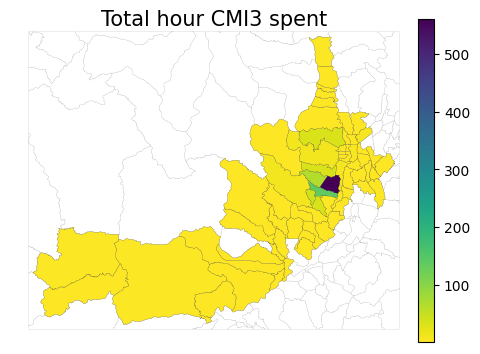
\includegraphics[width=.5\linewidth]{figures/map/CMI3_time.png}
        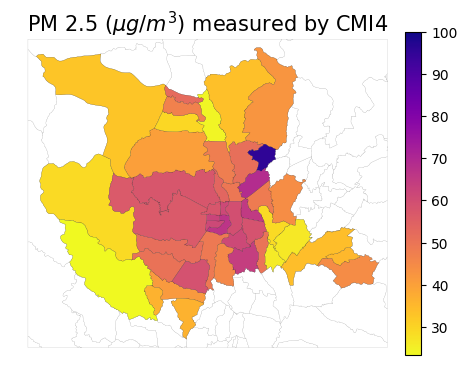
\includegraphics[width=.5\linewidth]{figures/map/CMI4_PM25.png}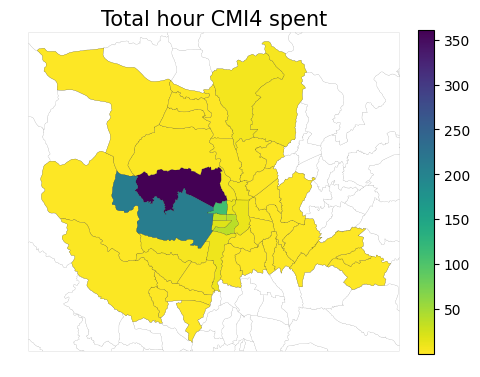
\includegraphics[width=.5\linewidth]{figures/map/CMI4_time.png}
        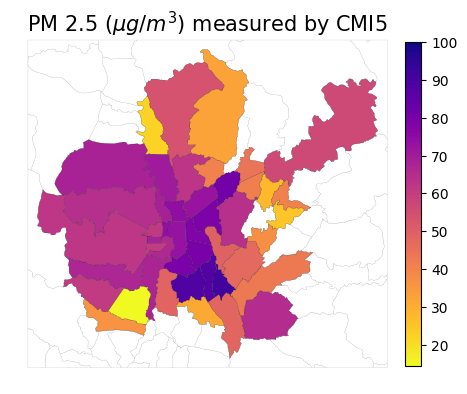
\includegraphics[width=.5\linewidth]{figures/map/CMI5_PM25.png}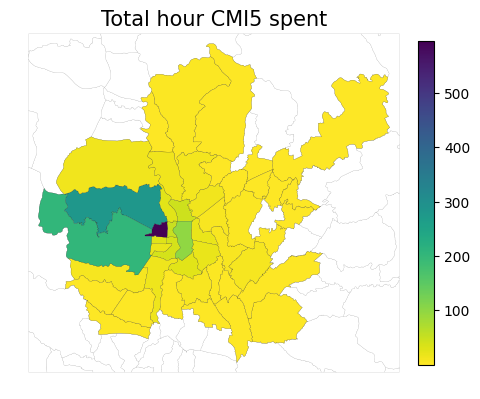
\includegraphics[width=.5\linewidth]{figures/map/CMI5_time.png}
        \caption{Measurement collected in Chiang Mai.}
\end{subfigure}\caption{
The left column of each sub-figure shows the average PM2.5 level throughout the study period measured in each subdistrict.
    The right column of each sub-figure shows the amount of time in hours that each driver spent in each subdistrict throughout the study.
}\Description{}
    \label{fig:subdistrict-aqi}\end{figure*} \subsection{Driver Responses to Air Pollution Exposure}
This section explores how drivers responded to the observed air pollution patterns, combining quantitative findings with qualitative insights from interviews and driver archetypes (``Income-Driven'' and ``Health-Conscious'').
While quantitative analysis reveals complex exposure patterns varying temporally (\autoref{fig:daily-pollution-per-driver}, \autoref{fig:hourly-work-aqi}) and spatially (\autoref{fig:subdistrict-aqi}) across individuals and cities,
driver responses show limited adaptation, dictated primarily by economic needs and the perceived unavoidability of pollution.

\subsubsection{Prioritizing Income Amidst Pervasive Pollution}
Our analysis reveals no correlation between drivers' daily work hours and concurrent average PM2.5 levels (\autoref{fig:work-hours-vs-aqi-per-rider}), indicating a lack of temporal work adjustments in response to pollution fluctuations.
This aligns with qualitative interviews where drivers frequently expressed perceiving pollution exposure as an unavoidable occupational hazard rather than a modifiable risk.
Many prioritized immediate income over avoiding polluted times, echoing sentiments like,

\begin{quoteb}
    ``I just go where the application tells me to go, ..., the (air) pollution is everywhere anyway\DIFdelbegin \DIFdel{'' (BKK-1}\DIFdelend \DIFaddbegin \DIFadd{.'' (BKK1}\DIFaddend )
\end{quoteb}

\begin{quoteb}
    ``When I see that the area gets smoggier, I often thought about driving out to the suburban area. But that means I'll have to drive an empty car out\DIFdelbegin \DIFdel{'' (BKK-5}\DIFdelend \DIFaddbegin \DIFadd{.'' (BKK5}\DIFaddend )
\end{quoteb}

This ``Income-Driven'' approach was common.
Driver \DIFdelbegin \DIFdel{BKK-1 }\DIFdelend \DIFaddbegin \DIFadd{BKK1 }\DIFaddend (46, Male), targeting 2,000-2,500 baht daily through long hours (4 AM-9 PM), exemplified this.
Despite experiencing symptoms like runny noses and eye irritation and becoming aware of pollution levels via our map visualization after joining the study, his driving patterns remained unchanged.
He explained his reliance on masks and persistence:

\begin{quoteb}
    ``I can feel my body gets weaker (the more I drive); I always wear masks. ... If Google Maps tells us to go, I go. Wherever it is, I just have to push through.'' (\DIFdelbegin \DIFdel{BKK-1}\DIFdelend \DIFaddbegin \DIFadd{BKK1}\DIFaddend )
\end{quoteb}

He further emphasized the lack of choice dictated by the platform and financial needs:

\begin{quoteb}
    ``I will not be able to be selective about routes; I go wherever the application assigns me to go, no matter of how far or how polluted the area may be.'' (\DIFdelbegin \DIFdel{BKK-1}\DIFdelend \DIFaddbegin \DIFadd{BKK1}\DIFaddend )
\end{quoteb}





The dominant narrative remains that immediate economic needs override pollution avoidance strategies concerning work timing.

\subsubsection{Limited Mitigation}
While prioritizing income was dominant, some drivers, exemplified by the ``Health-Conscious'' driver \DIFdelbegin \DIFdel{BKK-3}\DIFdelend \DIFaddbegin \DIFadd{BKK3}\DIFaddend , attempted mitigation strategies within existing constraints.
\DIFdelbegin \DIFdel{BKK-3 }\DIFdelend \DIFaddbegin \DIFadd{BKK3 }\DIFaddend (54, Female) actively incorporated heightened air pollution awareness into driving decisions after using the sensor helmet and map visualization.
She observed pollution spikes when riding behind buses,
\begin{quoteb}
    ``When I follow big buses, the graph just shoots up immediately.'' (\DIFdelbegin \DIFdel{BKK-3}\DIFdelend \DIFaddbegin \DIFadd{BKK3}\DIFaddend )
\end{quoteb}

and gained insight into hazardous AQI levels (80-100 \textmu{}g/m$^3$) even on seemingly clear days. This awareness prompted actions like avoiding main roads for side streets, despite potentially longer distances,
\begin{quoteb}
    ``Main roads have more dusts (air pollutants), it’s better to go through small alleys.'' (\DIFdelbegin \DIFdel{BKK-3}\DIFdelend \DIFaddbegin \DIFadd{BKK3}\DIFaddend )
\end{quoteb}

and selectively accepting rides or disabling auto-matching nearby to reduce prolonged exposure, particularly when heading home.



However, despite finding the real-time, localized AQI data useful, financial needs prevailed:

\begin{quoteb}
    ``We took this job for the money. We just have to live with it.'' (\DIFdelbegin \DIFdel{BKK-3}\DIFdelend \DIFaddbegin \DIFadd{BKK3}\DIFaddend )
\end{quoteb}

\DIFdelbegin \DIFdel{BKK-3}\DIFdelend \DIFaddbegin \DIFadd{BKK3}\DIFaddend 's experience illustrates the tension between health awareness and economic necessity.
While information tools provide valuable insights, platform constraints significantly limit drivers' ability to act on this information without sacrificing income.

\subsubsection{Increased Awareness and Community Engagement}
Participation in the study and access to the map visualization significantly increased drivers' awareness and spurred public engagement.
Most participants reported frequently checking the visualization, particularly on high-pollution days.
This led to discussions about air quality with friends and passengers; for instance, \DIFdelbegin \DIFdel{CMI-4 }\DIFdelend \DIFaddbegin \DIFadd{CMI4 }\DIFaddend advised others on mask use, while \DIFdelbegin \DIFdel{BKK-4 }\DIFdelend \DIFaddbegin \DIFadd{BKK4 }\DIFaddend shared real-time data from the visualization with passengers during rides in poor conditions.
The visualization thus served both as a personal reference tool and a catalyst for community awareness.

Driver \DIFdelbegin \DIFdel{CMI-1 }\DIFdelend \DIFaddbegin \DIFadd{CMI1 }\DIFaddend exemplified proactive community engagement.
He monitored morning pollution levels and actively shared warnings in the Chiang Mai \DIFdelbegin %DIFDELCMD < \grab{} %%%
\DIFdelend \DIFaddbegin \DIFadd{rideshare }\DIFaddend driver community (>5,000 members) when conditions were hazardous:

\begin{quoteb}
 ``I often take a screenshot (of the map visualization) when the air pollution levels turn red (hazardous) and share it in the group, warning everyone to be extra careful since the pollution got worsen that day.'' (\DIFdelbegin \DIFdel{CMI-1}\DIFdelend \DIFaddbegin \DIFadd{CMI1}\DIFaddend )
\end{quoteb}

This demonstrates how access to real-time, localized data empowered drivers beyond personal monitoring.
It fostered collective awareness and turned some participants, like \DIFdelbegin \DIFdel{CMI-1}\DIFdelend \DIFaddbegin \DIFadd{CMI1}\DIFaddend , into informal educators and active contributors to environmental health knowledge sharing within their community, moving beyond passive data reception.

\begin{figure*}
    \centering
    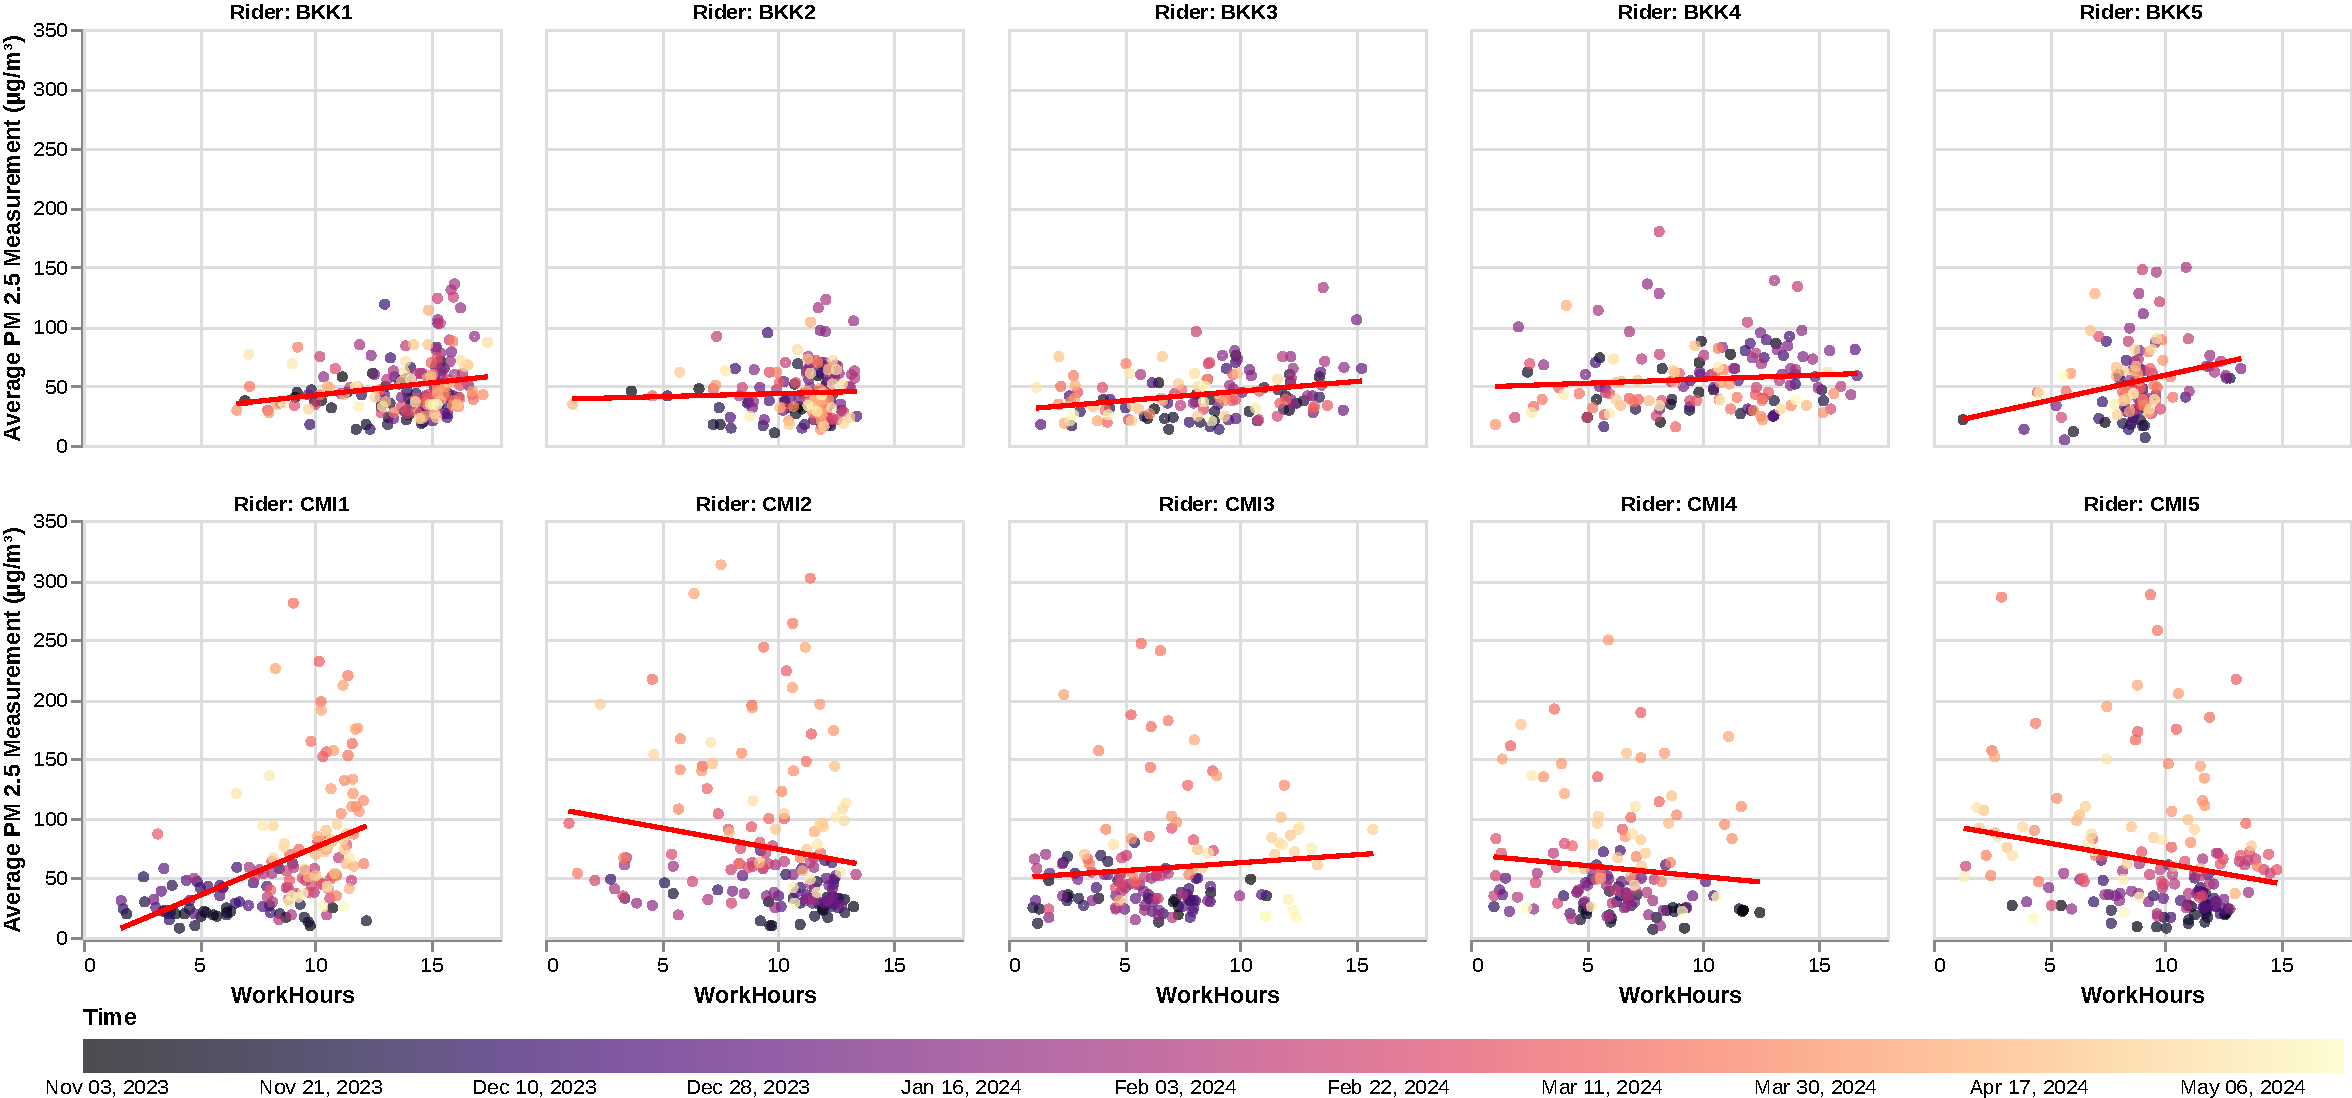
\includegraphics[width=\textwidth]{figures/work-hours-vs-aqi-per-rider-regression.pdf}
    \caption{Correlation of daily work hours and air pollution measurement for each driver, averaged through each week, with regression lines.
}
    \Description{}
    \label{fig:work-hours-vs-aqi-per-rider}
\end{figure*}

Overall, while access to air quality information increased awareness and even spurred community engagement, the demanding nature of gig work and the perceived ubiquity of pollution limit drivers' capacity to translate this awareness into significant behavioral changes, particularly regarding work schedules.
Financial imperatives largely override health considerations, highlighting the need for systemic interventions beyond individual information provision to effectively reduce exposure, such as low-emission zones or integrating real-time AQ data into traffic management. %
 \section{Discussion}

This study combines sensor data and interviews to offer a multi-modal perspective on Thai motorcycle rideshare drivers' experiences.
A key goal was understanding this environment to identify interventions improving driver health and livelihoods.
We discuss driver interest in real-time data, policy implications, infrastructure improvements, and platform-level incentives.

\DIFaddbegin \todo{what specific interventions-technological, regulatory, or organizational-do drivers themselves propose or prefer?}
\mick{I don't think they do?}
\mick{probably a better pay, but that does not solve the problem about the air pollution.}
\mick{they also said that they will drive no matter what}

\todo{How feasible are sensor-based early warning systems or adaptive work scheduling in practice?}
\mick{can say that participants are not bothered by the sensor?}
\mick{for charging, if we will be implementing this program, can we provide a battery charger to the driver? Maybe we can have a station to pick up / drop off a charger?}
\mick{may be we can add a paragraph here in the discussion section}

\todo{Are there gendered or age-related differences in exposure or agency?}
\mick{I think we have this data.}
\mick{Firn also brought this when we compared 2 types of drivers.}
\mick{If we don't want to make a point about gender / age, we can ignore this comment.}

\DIFaddend \para{User Interest in Real-Time Data}
Despite prior work~\cite{tieanklin2024rideshare} suggesting drivers prioritize revenue over technology-led behavioral change, participants valued real-time air quality data, feeling it empowered more informed decisions and increased awareness.
Drivers suggested integrating this data via motorcycle dashboards, ride-share apps, interactive maps, or directly into motorcycles.
Predictive algorithms could offer proactive warnings.
While designing non-distracting interfaces is challenging, this area warrants future investigation.



\para{Policy Interventions and Financial Support}
Government interventions like targeted financial support (e.g., subsidies for protective equipment, healthcare benefits, compensation during severe pollution) could improve driver outcomes.
Stricter emission controls and encouraging electric motorcycles offer long-term improvements.
Ultimately, reducing driver exposure requires a multi-stakeholder approach involving government, platforms, passengers, and drivers, integrating technology and policy to balance stakeholder needs (platform profitability, driver health/income, user convenience).

\para{Local and Collective Action}
The differing primary PM2.5 sources \DIFaddbegin \DIFadd{were }\DIFaddend identified; consistent traffic emissions in Bangkok versus seasonal agricultural burning dominating in Chiang Mai. 
This fundamentally shapes the air pollution challenge across regions and underscores that effective mitigation strategies must be location-specific. 
For instance, government policies like Work-From-Home (WFH) campaigns (e.g., Bangkok's 2024 initiative contributed to an 8\% traffic reduction  \cite{Wipatayotin_2025}) directly target the traffic congestion identified as Bangkok's primary issue, particularly during peak rush hours indicated by daily cycles (\autoref{fig:hourly-work-aqi}). 
Yet, these policies offer limited impact where sources differ (e.g., Chiangmai's burning season) and fail to resolve direct exposure for frontline workers like motorcycle taxi drivers who remain operational amidst pollution sources.
Therefore, effective solutions need integrated approaches by complementing national policies with targeted, local actions against dominant sources (traffic/burning) plus direct support (e.g., PPE, technology) for those highly exposed, potentially scaled through tailored public-private partnerships.











\para{Passenger Awareness and Platform-Level Incentives}
Ride-share platforms involve competing passenger and driver incentives.
For example, passenger demand for food deliveries during high pollution increases driver exposure.
Educating passengers about these risks could help.
Platforms could offer off-peak discounts during high-pollution events, aligning incentives, though potentially reducing platform usage.
Alternatively, external campaigns could discourage peak-pollution usage.















\para{Study Limitations}
Limitations include the sensor's battery power (8-10 hours), potentially causing data gaps during longer shifts despite recharge encouragement; direct motorcycle power is a future consideration.
Our non-random sample intentionally focused on uniquely deep, longitudinal lived experiences rather than generating statistically generalizable health conclusions typical of epidemiological studies.
Furthermore, sensors measured only a subset of pollutants, likely underestimating total exposure risks. \section{Conclusion}


This study investigated the severe PM2.5 exposure faced by motorcycle rideshare drivers in urban Thailand, 
highlighting how economic constraints create significant barriers for this population to follow standard health advice, even when aware of the dangers.
Building upon previously identified agency limitations, our seven-month mixed-methods study uniquely introduced a real-time air quality map visualization,
observing that although drivers incorporated this data to adjust routes and schedules,
income generation consistently superseded significant exposure mitigation actions.


Our contributions include fine-grained, individualized exposure data contextualized by lived experiences, revealing the complex interplay between health risks, economic pressures, and structural barriers.
The findings underscore the urgent need for multi-faceted interventions involving technology (e.g., real-time data interfaces), policy (e.g., financial support, targeted regulations), and platform adjustments.
%DIF < 
 %

\bibliographystyle{ACM-Reference-Format}
\bibliography{references}



\end{document}
